\documentclass[a4paper]{article}
\usepackage[utf8]{inputenc}
\usepackage[frenchb]{babel}
\usepackage{ifpdf}
\usepackage{graphicx} 
\usepackage{hyperref}
\title{Octochat \\ \textit{Le chat décentralisé}}
\author{Alexis \textsc{Giraudet} \and Benjamin \textsc{Sientzoff}}
\date{\today}
\ifpdf
\hypersetup{
    pdfauthor={Alexis Giraudet, Benjamin Sientzoff},
    pdftitle={Octochat - Discuter sur le réseau local sans serveur},
}
\fi
\begin{document}
	% page de garde avec sommaire
	\maketitle
	\vspace{5cm}
	\tableofcontents
	\newpage % passer à la page suivante
	
	\section*{Introduction}
		\paragraph{}{
		Ce projet a été réalisé dans le cadre du cours \textit{Objet et développement d'applications}
		dans lequel M. \textsc{Richoux} nous a enseigné l'utilisation des \textit{Design Patterns}.
		L'ambition de ce projet ne s'arrête pas là, car nous souhaitons poursuite le développement de notre 
		programme. Le sujet de notre projet est la création d'un client de chat qui n'utilise pas de serveur
		principal comme c'est le cas pour ce genre d'application réseau. Le fonctionnement est détaillé plus loin.
		}
		\paragraph{}{
		Octochat, notre programme, est donc un client de chat qui n'a pas besoin de serveur pour fonctionner.
		Lancer le programme, choisissez un nom d'utilisateur est c'est parti. Cependant, la mise en place d'une telle
		application n'est pas aisée. Ce rapport retrace la conception d'Octochat jusqu'au 26 novembre 2014. Il met en évidence les points qui ont posés problèmes et les différents \textit{patterns} utilisés.
		}
	
	\newpage
	
	\section{Utilisation et fonctionnement global}
	
		\paragraph{Boost}{
		Pour des questions de dépendances et pour faciliter le développement du programme, notamment pour ce qui est du réseau,
		nous avons choisi d'utiliser la librairie \textit{Boost}.
		L’utilisation de cette librairie nous permet également d'utiliser le système de compilation associé.
		}
	
		\subsection{Compilation du programme}
			\paragraph{Compilation}{
			Notre programme utilise deux bibliothèques à savoir la librairie standard du langage ( \textit{STL} et \textit{Boost}, plus précisément:
			\begin{itemize}
				\item[Boost.Build] le système de compilation (équivalant de \textit{make} et des \textit{Makefile} mais plus portable)
				\item[Boost.Thread] pour les \textit{thread]} et les \textit{mutex}
				\item[Boost.Log] pour les \textit{logs}
				\item[Boost.Asio] pour les entrées/sorties asynchrones sur le réseau
				\item[Boost.Serialization] pour sérialiser les données envoyées sur le réseau
				\item[Boost.System] pour les \textit{Smart Pointers} et le \textit{Lexical Cast}
			\end{itemize}
			}
			\paragraph{}{Pour compiler notre programme nous avons donc besoin d’un compilateur (incluant la \textit{STL}) et d’installer \textit{Boost}, c’est pourquoi nous avons réalisé un \textit{Makefile} qui s’occupe d’installer \textit{Boost} localement et de compiler le programme automatiquement.
			Une fois la compilation terminée, les exécutables sont placés dans le dossier \textit{build}:
			\begin{itemize}
				\item[octowatch] écoute le réseau
				\item[octoglobalchat] propose de chatter avec toutes les paires connectées
				\item[octochat] permet de chatter avec des utilisateurs
			\end{itemize}

			}
			\paragraph{Remarque}{
				Il est possible d’installer \textit{Boost} avec un gestionnaire de paquets à condition d’avoir les privilèges suffisants.
			}


			\paragraph{}{
				Pour compiler le projet, on commence par cloner le dépôt, puis on lance la commande make à la racine du projet.
			}
			
			\begin{verbatim}
				$ git clone https://github.com/blasterbug/Octochat.git
				$ cd Octochat
				$ make
			\end{verbatim}
		
		\subsection{Utilisation}
			\paragraph{}{
			Si toutes les précédentes étapes se sont bien passées, vous êtes maintenant en mesure d'utiliser Octochat.
			Pour lancer l'application taper simplement \verb|./octochat|
			}
		
		\subsection{Sous le capot}
			\paragraph{}{
			Dès le début, nous avons décidé de diviser notre application en couches.
			Une première couche s'occupe de la gestion du réseau à proprement parler. Une seconde couche, qui pourrait être découper elle aussi en deux parties s'occupe des aspect applicatif du programme.
			}
			
			\paragraph{Couche réseau}{
			C'est la partie du programme la plus critique et la plus difficile à mettre en œuvre.
			Le serveur, \textit{octonet} qui tourne en local sur chaque client, utilise deux \textit{threads}.
			Le premier permet d'écouter sur un premier port. L'écoute de ce port assure le maillage des pairs local. 
			En effet, à chaque fois qu'un pair arrive, une tram réseau est envoyé sur ce port en \textit{broadcast}. On peut ainsi maintenir une liste des pairs connectées.
			Le second \textit{thread} écoute un second port qui permet de recevoir des requêtes réseau permettant de 
			transmettre des données une fois qu'on connaît les paires locales. Ces requêtes permettent notamment à 
			la couche de plus au niveau de mettre en place un protocole, \textit{octochat protocol}. Un protocole
			spécialement conçu pour notre programme.
			}
			
			\paragraph{Couche applicatif}{
			La couche applicatif permet de définir un protocole sur lequel Octochat peut reposer permettant ainsi 
			de gérer les utilisateurs d'un salon (une \textit{octoroom}), leur connexion et leur déconnexion au sein
			des salons.
			}
		\newpage
		
	\section{Patrons de conception}
			% diagramme UML 
			% parapgraphes qui explique le pourquoi du comment
		\subsection{Observer}
		\subsection{Factory method}
		\subsection{State}
			\paragraph{}{
			Le \textit{pattern state} nous a permis de gérer la connexion des utilisateurs.
			}
			\begin{center}
				\begin{figure}
					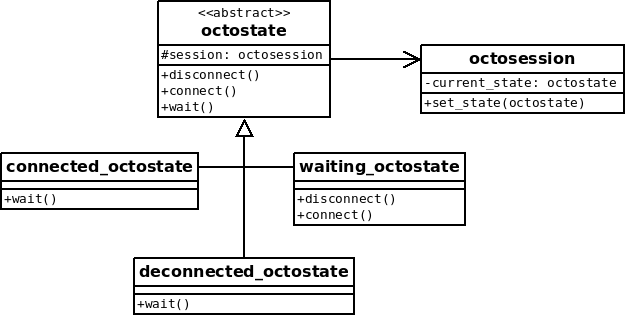
\includegraphics[scale=0.6]{UML/state.png}
					\label{state_uml}
					\caption{Diagramme UML du \textit{pattern state}}
				\end{figure}
			\end{center}
	\newpage
	
	\section*{Conclusion}
		\paragraph{}{je conclu}
		
\end{document}
